% 先端芸術音楽創作学会会報テンプレート ver.200908
% By Daichi Ando
% based on ICMC2005

\documentclass{jsarticle}
\renewcommand{\baselinestretch}{0.9}
\usepackage{url}
\usepackage{ascmac}
\usepackage{jssa,amsmath}
\usepackage{mediabb}
\usepackage{listings,jlisting}
\usepackage{graphicx}
\usepackage{plext}
\usepackage{setspace}
\usepackage{color}
\usepackage{setspace}

\definecolor{mygray}{rgb}{0.9,0.9,0.9}

\lstset{%
 backgroundcolor=\color{mygray},
 basicstyle={\small\ttfamily},%
 stringstyle={\small},
 breaklines=true,
 columns=[l]{fullflexible},%
 frame={l},
 numbers=left,%
 tabsize=3,%
 xrightmargin=0zw,%
 xleftmargin=0zw,%
 numberstyle={\scriptsize},%
 stepnumber=1,
 numbersep=1zw,%
 lineskip= -0.5zw%
}

\def\boutenchar{・}
\def\lstlistingname{リスト}

% Title.
% ------
% LaTeX環境によっては,maketitleでエラーが出ることもあるが,強行して良い

\title{Super Collider チュートリアル (2)\\ 
Super Collider Tutorials (2)
}

% Paper Category 論文,報告,連載,書評……など
\category{連載}

% Single address
% To use with only one author or several with the same address
% ---------------
\oneauthor
  {美山 千香士\\Chikashi Miyama} 
  {ケルン音楽舞踏大学\\Hochschule f\"{u}r Musik und Tanz K\"{o}ln} 

\begin{document}

%%% --ページ数等の指定
\makeatletter 
\def\ps@myheadings{% 
\let\ps@jpl@in\ps@plain% 
\def\@evenhead{\reset@font\hfil\leftmark\hfil}% 
\def\@oddhead{\reset@font\hfil\rightmark\hfil}% 
\let\@mkboth\@gobbletwo% 
\let\sectionmark\@gobble% 
\let\subsectionmark\@gobble% 
% 
\def\@oddfoot{\reset@font\hfil-- \thepage --\hfil}% 
\let\@evenfoot\@oddfoot 
} 
\makeatother 

%%% 
%%% 開始ページ数を設定する 
%投稿の段階では無視

\setcounter{page}{ 9 } 
\pagestyle{myheadings} 

%%% 
%%% 論文のVol., No., pp.を設定する 
% 投稿の段階では無視

\markright{\footnotesize \gt 先端芸術音楽創作学会 会報 Vol.1 No.1 pp.9--16 }

%%% 
%%% \maketitleの直後の行に \thispagestyle{myheadings} を挿入する。 

\maketitle
\thispagestyle{myheadings}

%
\begin{abstract}
 本連載では、リアルタイム音響合成環境のSuperCollider(SC)の使い方を、同ソフトを作品創作や研究のために利用しようと考えている音楽家、メディア・アーティストを対象にチュートリアル形式で紹介する。\\
SuperCollider(SC) is a realtime programming environment for audio synthesis. This article introduces SC to musicians and media artists who are planning to utilize the software for their artistic creations and researches.

\end{abstract}
%
\section{今回の目標:SCによるメロディの演奏}
前回はSC\cite{scsite}のインストール、ソフトウェアの構成、音の出し方などのプログラミングの基礎を勉強した。今回は、前回の内容を発展させ、簡単なメロディを自動的に演奏するプログラムを作り、それを通してSCで音楽を作る上で必要不可欠な以下の3項目を順に学習していく。

\begin{itemize}
 \item {\bf Env}と{\bf EnvGen}を用いた「音符」作り
 \item {\bf SynthDef}を用いた「楽器」作り
 \item {\bf Routine}を用いた「楽譜」作り
\end{itemize}

\section{「音符」を作る}
前回、SinOscなどのUGenを用いてSCで音を出す方方法を学習したが、それらはストップコマンド[Cmd+.]などで強制的に終了させない限り音が止まらない「持続音」であった。これでは今回の目標である「メロディ」を演奏するのは難しい。故に、まずはじめに一定時間で発音が止まる音価のある音、
「音符」を作る必要がある。このためにSCでは{\bf エンベロープ}を用いる。エンベロープを作るには{\bf Env}というクラスと{\bf EnvGen}というUGenを組み合わせる。Envはエンベロープの「設計」を行い、EnvGenはEnvを使って設計したエンベロープを生成し、音に適用できるようにする役割を担う。

\subsection{エンベロープの設計}
SCでは、エンベロープは、目標とする値とその値に達する推移時間の組み合わせによって定義する事ができる\footnote{本稿では音の長さの決まった固定長のエンベロープのみを扱うが、可変長のエンベロープを用いる事も可能である。この場合はEnv.adsrとEnv.asrなどによりエンベロープを定義する。詳しくはEnvのヘルプファイルを参照のこと。}。例えば、リスト\ref{code:env}は、Envを用いて0.5秒のアタックと1秒のサステイン、0.5秒リリースのみの簡単なエンベロープを設計したものである。
\begin{lstlisting}[caption=エンベロープの設計,label=code:env]
Env.new([0,1,1,0],[0.5,1.0,0.5]).plot;
\end{lstlisting}
Envを使ってこのようにエンベロープを設計し、.plotというメッセージを送ると、エンベロープがプロット(図示)される。Envの第1引数の[ ]の中の数値がそれぞれエンベロープのノード(節点)の値を、続く第2引数の[ ]内の数値がノード間の時間を指定している(図\ref{fig:plot})。

\begin{figure}[htbp]
 \begin{center}
  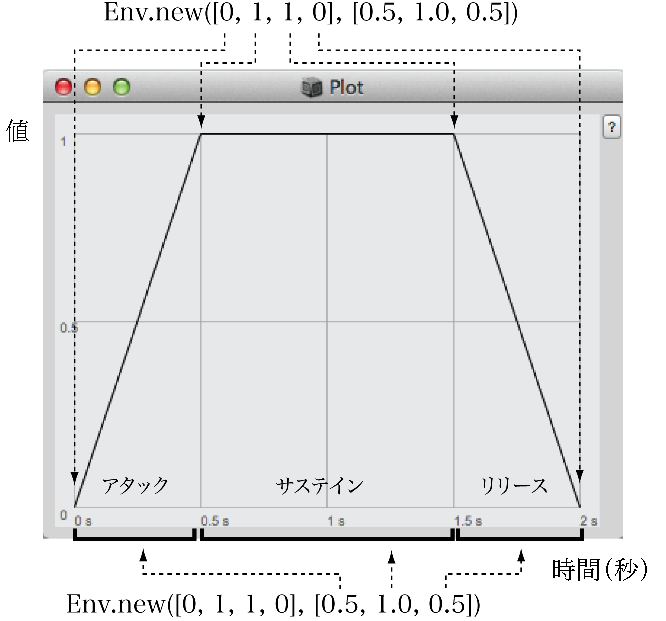
\includegraphics[scale=0.6]{plot_env.pdf}
 \end{center}
 \caption{エンベロープ}
 \label{fig:plot}
\end{figure}

また、リスト\ref{code:test}のように、さらに.testを.plotの前に挟むと、自動的にSCがこのエンベロープを正弦波の振幅に適用したものを試奏するので、エンベロープを聴感で吟味したいときに便利である。尚、.testを使う時はSC Serverを事前に起動する必要がある。

\begin{lstlisting}[caption=.testの利用,label=code:test]
e=Env.new([0,1,1,0],[0.5,1,0.5]);
e.test.plot;
\end{lstlisting}

\subsection{Array-複数のデータをまとめて保存する}
リスト\ref{code:env}で、Envは2つの引数を与えられているが、そのいずれもが[ ]に囲まれ、その中に複数の数値が列挙されている。このようにSCでは、複数のデータをコンマで区切って列挙し、[ ]で囲ったものをArray(配列)という。Arrayは複数のデータを集合として扱うときに重宝する。例えば、リスト \ref{code:array}の1行目の[5,8,2,4,9]は5つの数値をArrayを用いてひとまとめにしている。
\begin
{lstlisting}[caption=Arrayの例,label=code:array]
a=[5,8,2,4,9];
a.at(3);
\end{lstlisting}
Arrayは数値などと同様に、変数に代入する事ができるため、複数のデータをまとめて1つの変数名で扱えるという利点がある。変数に代入したArrayの{\it n}番目の要素を参照するには、リストの2行目のようにArrayを格納した変数に.at({\it n})を送る。図\ref{fig:index}の示すように、Array内の要素のインデックス(カウント)は0から始まるため、.at(3)を送るとArrayから4が返される。SCでは実行したコードの最終行の評価結果が自動的にポスト・ウインドウに表示されるので、リスト\ref{code:array}を実行するとポスト・ウインドウに「4」が表示される。

\begin{figure}[htbp]
 \begin{center}
  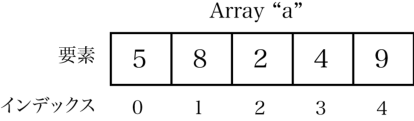
\includegraphics[scale=0.9]{index.pdf}
 \end{center}
 \caption{Arrayの要素とインデックスの関係}
 \label{fig:index}
\end{figure}

Array内の各要素を順番に参照し、ポスト・ウインドウに表示させる場合は、リスト\ref{code:itteration}のように記述する。Arrayの.doを実行すると、.doの引数として渡された\{\}で囲まれたコードが、Arrayの要素数の回数(この場合は5回)繰り返し実行される。関数が実行される度に、引数itemにはArrayの各要素が順番に代入される。このように.doを使ってArray内の各要素を順番に評価していく手法を{\bf イテレーション}という。
また、プログラム中のitem.postlnは「itemの中身をポスト・ウインドウに表示せよ」という意味である。前述のように、プログラムの最後に実行したコードの評価はポスト・ウインドウに自動的に表示されるが、そうでない場合は、このように.postlnを使って強制的にポスト・ウインドウへの表示を促すことができる。

\begin{lstlisting}[caption=イテレーション,label=code:itteration]
a = [5,8,2,4,9];
a.do({
  arg item;
  item.postln;
});
\end{lstlisting}

Arrayには、整数や少数などの数値だけでなく、リスト\ref{code:mixed}のように様々なタイプのデータを混ぜて格納することも可能である。さらに、Arrayの中にArrayを入れ子のように格納することもできる。このような場合は、リスト\ref{code:mixed}の2行目のように、a.at(3)でArray a のインデックス3の要素、[2,10,-1]を参照し、それにさらに.at(2)を送ることで、Arrayの中のArrayのインデックス2の要素、-1を取り出す事ができる。

\begin{lstlisting}[caption=Arrayに数値以外のものを格納する,label=code:mixed]
a=["JSSA",-17,0.995,[2,10,-1]];
a.at(3).at(2);
\end{lstlisting}

Arrayは.atの他にも様々な命令を受けつける、例えば.sumはArray内の全ての要素の合計を計算、.sortはArray中の要素を昇順に並べ替え、.rotateはArrayの要素を()で指定した数だけArrayの最後尾から先頭に移動、.indexOfは()内で指定した要素がArrayの何番目に格納されているのかを返す(リスト\ref{code:flex_array})。5行目のように、Array対して四則演算を行う事も可能で、この場合はArray内の全ての要素に10が加算され、Arrayが[15,18,12,14,19]となる。

\begin{lstlisting}[caption=Arrayの受け付ける様々な命令,label=code:flex_array]
[5,8,2,4,9].sum.postln;
[5,8,2,4,9].sort.postln;
[5,8,2,4,9].rotate(2).postln;
[5,8,2,4,9].indexOf(9).postln;
([5,8,2,4,9]+10).postln;
\end{lstlisting}

\begin{itembox}[l]{Env}
{\footnotesize 
エンベロープを設計するためのクラス。\\\\
.new({\it levels}, {\it times}, {\it curve}, {\it releaseNode}, {\it loopNode}, {\it offset})\\

{\it levels} $\cdots$エンベロープのノードの値。Arrayで指定する\\
{\it times} $\cdots$ノード間の補間時間。Arrayで指定する\\
{\it curve} $\cdots$ノード間の補間方法。\\
(残りの引数の解説はヘルプファイルを参照のこと)
}
\end{itembox}

\subsection{エンベロープの適用}
さて、Arrayの役割と使用法を学んだので、次にArrayを使って設計したエンベロープを使って音作りを行う。エンベロープを音に適用するには、{\bf EnvGen}というUGenを用いてエンベロープをオーディオ信号として生成し、それを適用の対象となる信号と乗算する。リスト\ref{code:apply}はSaw.arを使って生成したノコギリ波にEnvで設計したエンベロープをEnvGenを用いて適用したものである。

\begin{lstlisting}[caption=エンベロープの適用,label=code:apply]
{
  e=Env.new([0,1,1,0],[0.5,1,0.5]);
  Saw.ar(880,0.1)*EnvGen.ar(e);
}.play;
\end{lstlisting}

\begin{itembox}[l]{EnvGen}
{\footnotesize 
エンベロープを生成するUGen。\\\\
.ar({\it envelope}, {\it gate}, {\it levelScale}, {\it levelBias},{\it timeScale}, {\it doneAction})\\
.kr({\it envelope}, {\it gate}, {\it levelScale}, {\it levelBias},{\it timeScale}, {\it doneAction})\\

{\it Env} $\cdots$Envによって設計したエンベロープ\\
{\it gate} $\cdots$ゲート値。0より大きい値が入力されるとエンベロープの生成を開始する\\
{\it levelScale} $\cdots$レベルの伸縮値\\
{\it levelBias} $\cdots$レベルのオフセット値\\
{\it timeScale} $\cdots$エンベロープの補間時間の伸縮値\\
{\it doneAction} $\cdots$エンベロープ終了時の処理を指定する値\\
}
\end{itembox}

\subsection{エンベロープ終了時の処理指定-doneAction}
SCウインドウの右下にあるステータス・バーは現在のサーバの状況を表示しており、左から順番に「CPU使用率(平均)」「CPU使用率(ピーク)」「使用中のUGen数」「使用中のSynth数」「使用中のGroup数」「定義されたSynthDef(後述)の数」が表示されている(図\ref{fig:booted})。この図のステータス・バーはサーバを立ち上げた直後のもので、何も演奏していないので、UGenの数が0uとなっている。

\begin{figure}[htbp]
 \begin{center}
  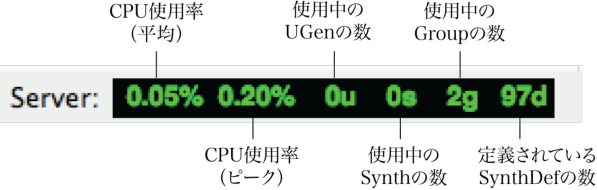
\includegraphics[scale=0.8]{booted_comment.pdf}
 \end{center}
 \caption{ステータス・バーの項目}
 \label{fig:booted}
\end{figure}

リスト\ref{code:apply}を実行すると、SCのステータスバーが、11u、1s、2gを表示し、プログラムが、いくつかのUGenを使って音を生成しているのが分かるが\footnote{リストではEnvGenとSawの2つのUGenしか使用していないが、ステータスバーには11uと表示される。これは、SCが適切なオーディオ・チャンネルに音を送る処理などのために自動的に幾つかのUGenを使うためである。後述するSynthDefを用いた場合は、リスト中のUGenの数とステータス・バーのUGenの数は一致するようになる。}、2秒後にエンベロープが終わり、無音状態になっても、この表示が変わらず、UGenを使い続けており、SCが無用な計算を続けていることがわかる(図\ref{fig:status})。

\begin{figure}[htbp]
 \begin{center}
  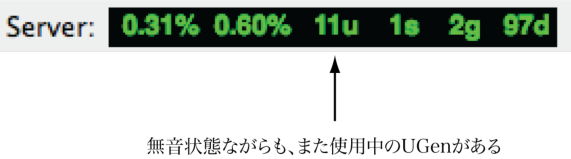
\includegraphics[scale=0.8]{status_comment.pdf}
 \end{center}
 \caption{エンベロープ開始から2秒以降のステータス}
 \label{fig:status}
\end{figure}

このようなリソースの無意味な消費を回避するために、エンベロープが終了すると同時にSCに計算を停止させる必要がある。これを行うにはEnvGenの引数の末尾に{\bf doneAction:2}を加え、リスト\ref{code:doneAction}のように変更する。このコードを実行すると、発音の開始から2秒後にUGenの数が11uから0uに自動的に変化し、発音のために使用したUGenがエンベロープの終了に同期して解放されたのが分かる。

 \begin{lstlisting}[caption=doneActionを指定,label=code:doneAction]
{
  e=Env.new([0,1,1,0],[0.5,1,0.5]);
  Saw.ar(880,0.1) * EnvGen.ar(e,doneAction:2);
}.play;
\end{lstlisting}

このようにエンベロープの終了(done)の時の振る舞い(Action)を設定するのがdoneActionである。これに「2」を指定する事により、終了と同時にこの音に関するプロセスを停止するので、無用な計算リソースの消費を防ぐ事が可能になる。doneActionには2以外にも0から14までの数を与える事で、終了時の振る舞いを様々に指定する事ができる。詳しくはヘルプファイル、「UGen done-actions」を参照されたい。

\subsection{キーワードによる引数の指定}
前項において、「doneAction:2 」という特殊な表記によってEnvGenの引数を指定した。SCでは、UGenなどに引数を渡すときには、リスト\ref{code:normal_args}のように、それぞれの引数が何のパラメータをコントロールするのかをヘルプファイルで調べ、順番に引数を渡していくのが一般的である。
\begin{lstlisting}[caption=一般的な引数の指定,label=code:normal_args]
{
  SinOsc.ar(880,0.0,0.1,0.0);
}.play;
\end{lstlisting}

例えば、リスト\ref{code:normal_args}において、SinOsc.arの引数はfreq, phase, mul, addであるので、SinOsc.ar(880, 0.0, 0.1, 0.0)のように書くことでそれぞれfreq = 880, phase = 0.0, mul = 0.1, add = 0.0 を指定できる。だが、{\bf キーワード}(引数の名前)を使って特定の引数だけを設定する事もできる。キーワードですべてのパラメータを指定した場合は、引数の順番に留意する必要がなくなる。例えばリスト\ref{code:kwd_args}では、freqの前にmulを指定しているが、正常に作動する。

\begin{lstlisting}[caption=キーワードによる引数の指定,label=code:kwd_args]
{
  SinOsc.ar(mul:0.1,freq:880);
}.play;
\end{lstlisting}

また、リスト\ref{code:hashed}のように順番に引数を与えていく手法とキーワードによる引数の指定は混在してもかまわない。だが、この場合キーワード指定でない引数は、必ず順番に先頭から記述する必要がある。

\begin{lstlisting}[caption=引数指定法の混在,label=code:hashed]
{
  SinOsc.ar(880,mul:0.1);
}.play;
\end{lstlisting}

リスト\ref{code:doneAction}のEnvGen.ar(e, doneAction:2)は、このように2つの引数の指定方法を混在させた例である。UGenにはEnvGenのように非常に多くの引数をとれるものもあり、その際にこの事を知っていると、より簡潔かつ柔軟にプログラムを書くことができる。

\subsection{エンベロープの応用}
エンベロープはオシレータからの波形の振幅をコントロールする使い方が最も一般的だが、これ以外にも例えば周波数や、フィルタのパラメータをコントロールする事もできる。リスト\ref{code:pitch}では、ノコギリ波の周波数の上げ下げをエンベロープを用いて行っている。このように、エンベロープはさまざまなパラメータのコントロールに柔軟に利用できる。

\begin{lstlisting}[caption=エンベロープの応用,label=code:pitch]
{
  e=Env.new([220,880,440],[1,0.5]);
  Saw.ar(EnvGen.ar(e, doneAction:2), 0.1);
}.play;
\end{lstlisting}

\section{「楽器」を作る}
\subsection{自分だけの楽器を定義する-SynthDef}
これまで勉強してきたように、SCでは様々なUGenを組み合わせて、独自の音作りをすることができる。そして、SCには気に入った音が出るプログラムを自分独自の{\bf Synth}(楽器)として定義・保存し、定義したSynthを様々な作品で再利用できる仕組みが用意されている\footnote{SCでは今回の例のように発音を担うものはもちろん、エフェクタ、アナライザー、ミキサーなど様々なものをSynthとして定義できる}。

Synthを定義するには、リスト\ref{code:synthdef}の要領で{\bf SynthDef}を使う。SynthDefとは文字通りSynthを定義(Define)するクラスで、第1引数("jssa1")でそのSynthの名前を設定し、第2引数はそのSynthを定義する。この定義の中で使われているUGen、{\bf Out}は音を送る先のチャンネルを指定している。リストの4行目のように、Outの第2引数にUGenを代入した変数を指定し、第1引数に0を指定すると左チャンネルに、1を指定すると右チャンネルに音を送る設定となる。

\begin{lstlisting}[caption=SynthDefの使用,label=code:synthdef]
SynthDef.new("jssa1", {
  a=Saw.ar(440,0.1);
  e=Env.new([0,1,1,0],[0.05,0.1,0.1]);
  Out.ar(0,a*EnvGen.ar(e, doneAction:2));
}).load;
\end{lstlisting}

定義したSynthを実際に生成して使用するにはリスト\ref{code:synth_use}のように、SynthDefで定義したSynthの名前をSynthの第1引数に指定する。
\begin{lstlisting}[caption=定義したSynthを使う,label=code:synth_use]
Synth.new("jssa1");
\end{lstlisting}

現段階では、このSynthは440Hzの音しか出せないが、Synthの周波数を自由に設定・変更できるようにすることもできる。そのためには、SynthDefの中にargを用いてfreqという引数をリスト\ref{code:synth_with_args}のように宣言する。このようにargを使うと、Synthが外部から引数を取る事ができるようになる。

\begin{lstlisting}[caption=SynthDefの使用法,label=code:synth_with_args]
  SynthDef.new("jssa2",{
    arg freq;
    a=Saw.ar(freq, 0.1);
    e=Env.new([0,1,1,0],[0.05,0.1,0.1]);
    Out.ar(0,a*EnvGen.ar(e,doneAction:2));
  }).load;
\end{lstlisting}

周波数を指定してSynthを使用するには、Synthの第2引数としてArrayを与え、その中に「引数名」「数値」のペアを記述する。

\begin{lstlisting}[caption=argの指定,label=code:synth_with_args_use]
Synth.new("jssa2",["freq",880]);
\end{lstlisting}

これを応用すれば、和音をSCに演奏させるなども容易である。例えば以下の3行を選択し、同時に実行すれば長三和音が生成される。
\begin{lstlisting}[caption=和音,label=code:chord]
Synth.new("jssa2",["freq",60.midicps]);
Synth.new("jssa2",["freq",64.midicps]);
Synth.new("jssa2",["freq",67.midicps]);
\end{lstlisting}

argはSynthDefの中で複数個宣言する事もできる。リスト\ref{code:synth_with_two_args}のSynthDefでは周波数の他に振幅もargを介して指定できるようにしている。それぞれのargを指定するにはリスト\ref{code:synth_with_two_args_use}のように、Synthの第2引数のArray内に引数名と値を列挙していく。また、SynthDef内で、argにはfreq = 440, amp = 0.1のように初期値を設定しておくことができる。この初期値はargに対しパラメータが与えられなかった時に用いられる。

\begin{lstlisting}[caption=SynthDefの使用法,label=code:synth_with_two_args]
SynthDef.new("jssa3",{
   arg freq = 440,amp = 0.1;
   a=Saw.ar(freq,amp);
   e=Env.new([0,1,1,0],[0.05,0.1,0.1]);
   Out.ar(0,a*EnvGen.ar(e,doneAction:2));
}).load;
\end{lstlisting}
\begin{lstlisting}[caption=argの指定,label=code:synth_with_two_args_use]
Synth.new("jssa3",["freq",880,"amp",0.5]);
\end{lstlisting}

\begin{itembox}[l]{Out}
{\footnotesize 
信号の出力先のバスを指定するためのUGen\\\\
.ar({\it bus}, {\it channelsArray})\\
.kr({\it bus}, {\it channelsArray})\\

{\it bus} $\cdots$出力先のバス\\
{\it channelsArray} $\cdots$バスに送る信号。複数の信号を送る場合はArrayを渡す。Arrayが渡された場合、{\it bus}で指定されたバスから順番に信号が送られる。バスの概念については回を改めて詳説する。
}
\end{itembox}

\subsection{SynthDefファイル}
SynthDefを用いてSynthを命名、定義した後に、定義したSynthをSCサーバに登録する必要がある。リスト\ref{code:synth_with_two_args}の最後の.loadメッセージは、SCサーバへの登録を行うためのコマンドであり、これを指定しないと定義したSynthを使う事はできない。

また、一度SynthDefに.loadを送ると、その定義が書かれたSynthDefという定義ファイルが、Macでは「$\sim$/Library/Application Support/SuperCollider/synthdefs」に保存される。一度ここに保存されたSynthDefはSCサーバを再度立ち上げた時に自動的にサーバに登録され、再定義する必要なくなる。このため、自分の気に入った音を出すSynthを予め定義し、SynthDefファイルに保存しておくと、複数のプロジェクトで1つのSynthを流用する事などが容易となる。

このように.loadを送ると、SCサーバへのSynthの登録と、SynthDefファイルへの定義の書き出しが同時に行われるが、SynthDefで定義したSynthをSynthDefファイルを保存することなく、使用したい場合は、.loadメッセージの代わりに.sendを送る(図\ref{fig:load_send})。

\begin{figure}[htbp]
 \begin{center}
  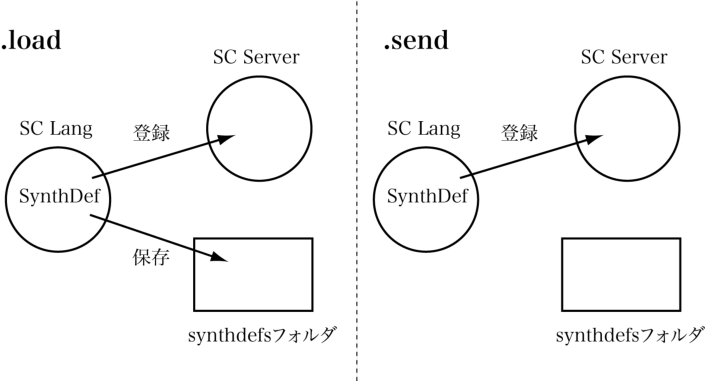
\includegraphics[scale=0.7]{SynthDef.pdf}
 \end{center}
 \caption{.loadと.sendの違い}
 \label{fig:load_send}
\end{figure}


\begin{itembox}[l]{SynthDef}
{\footnotesize 
Synthを定義し、保存するためのクラス。\\\\
.new({\it name}, {\it ugenGraphFunc}, {\it rates}, {\it prependArgs}, {\it variants}, {\it metadata})\\

{\it name} $\cdots$名称。Synthにより参照される\\
{\it ugenGraphFunc} $\cdots$Synthの定義\\
(全ての引数はヘルプファイルを参照のこと)
}
\end{itembox}

\begin{itembox}[l]{Synth}
{\footnotesize 
SynthDefで定義したSynthを使用する際に用いる。\\
.new({\it defname}, {\it args}, {\it target}, {\it addAction:'addToHead'})\\

{\it name} $\cdots$事前に定義したSynthDefの名称\\
{\it args} $\cdots$Synthに渡すパラメータを列挙したArray\\
(全ての引数はヘルプファイルを参照のこと)
}
\end{itembox}

\section{「楽譜」を作る}
前項で「楽器」をSynthとして定義した事で、より柔軟に任意の音のパラメータをコントロールできるようになったので、あとはこのSynthの発音のタイミングを時間軸上にスケジュールする、いわば「楽譜」をプログラムする事で、SCにメロディを奏でさせることが可能となる。

\subsection{任意のタイミングで音を出す-Routine}
SCでユーザの任意の時間に音が鳴るようにするには{\bf Routine}を使う。使い方は、リスト\ref{code:routine}のようにRoutineの引数の\{\}の中にSynthを使った発音を促すコードを書き、その間に処理を遅延させる.waitを挟んでいく。

\begin{lstlisting}[caption=Routineの使用,label=code:routine]
Routine({
  Synth.new("jssa3",["freq",60.midicps]);
  0.5.wait;
  Synth.new("jssa3",["freq",64.midicps]);
  1.0.wait;
  Synth.new("jssa3",["freq",67.midicps]);
}).play;
\end{lstlisting}

リスト\ref{code:routine}を実行すると、MIDIノート・ナンバーの「60」、つまりピアノの真ん中のドが演奏され、その0.5秒後に64(ミ)、そのさらに1秒後に67(ソ)が演奏される。このように.waitを使って処理を遅延させる事で任意のタイミングでSCに発音を促す事が可能となる。

\subsection{旋律を演奏する}
リスト\ref{code:mary}は上記のRoutineを利用して「メリーさんの羊」の冒頭部分を演奏するプログラムである。

\begin{lstlisting}[caption=メリーさんの羊,label=code:mary]
Routine({
  a = [[69,0.3],[67,0.1],[65,0.2],[67,0.2],
[69,0.2],[69,0.2],[69,0.2]];
  a.do({
    arg item;
    Synth.new("jssa3",["freq",item.at(0).midicps]);
    item.at(1).wait;
  });
}).play;
\end{lstlisting}

リストの冒頭では、各音のMIDIノートナンバーと音価のペアを複数のArrayとして宣言し、それをさらにArray、aに格納している。そして、Array aの各要素を上述した.doを用いたイテレーションの手法を使って、順番に参照しており、itemは[69, 0.3], [67, 0.1], [65, 0.3]...という順番でピッチと音価のペアのArrayに置き換えられる。そしてitemの0番目の要素=ピッチのデータはSynthに渡され、1番目の要素=音価のデータは.waitに用いられているため、任意のピッチの音を任意のタイミングに鳴らすこと、つまりメロディーを奏でる事が可能となっている。

\subsection{移調・テンポチェンジ}
「メリーさんの羊」はリスト\ref{code:mary}ではヘ長調であるが、リスト\ref{code:transpo}のようにitem.at(0)の後に-6を追加する事によって、半音階で6度下のハ長調に移調する事もできる。また、このコードではitem.at(1)に1.5を乗算し、.waitによる待機時間を延ばすことによって、テンポを遅くしている。
\begin{lstlisting}[caption=移調,label=code:transpo]
Routine({
  a = [[69,0.3],[67,0.1],[65,0.2],[67,0.2],
    [69,0.2],[69,0.2],[69,0.2]];
  a.do({
    arg item;
    Synth.new("jssa3",["freq",(item.at(0)-6).midicps]);
    (item.at(1)*1.5).wait;
  });
}).play;
\end{lstlisting}

このように若干の変更をプログラムに加えることで、音楽の特徴を大幅に変化させることが出来るところが、SCで音楽を作る醍醐味の1つといえるだろう。

\section{謝辞}
本稿の執筆にあたり、校正を手伝って頂いた理化学研究所・岡ノ谷情動情報プロジェクトの濱野峻行氏に心からの感謝の気持ちとお礼を申し上げたい。

\bibliographystyle{jplain}
\begin{thebibliography}{citations}
  \bibitem{scsite} {\it SuperCollider}, \url{http://supercollider.sourceforge.net/}(アクセス日 2013年7月3日)
\end{thebibliography}

\section{著者プロフィール}
\subsection*{美山 千香士 (Chikashi Miyama)}
作曲家、電子楽器創作家、映像作家、パフォーマー。国立音楽大学音楽デザイン学科より学士・修士を、スイス・バーゼル音楽アカデミーよりナッハ・ディプロムを、アメリカ・ニューヨーク州立バッファロー大学から博士号を取得。Prix Destellos特別賞、ASCAP/SEAMUS委嘱コンクール2位、ニューヨーク州立大学学府総長賞、国際コンピュータ音楽協会賞を受賞。2004年より作品と論文が国際コンピュータ音楽会議に12回入選、現在までに世界18カ国で作品発表を行っている。 2011年、DAAD(ドイツ学術交流会)から研究奨学金を授与され、ドイツ・カールスルーエのZKMで客員芸術家として創作活動に従事。近著に「Pure Data-チュートリアル&リファレンス」(Works Corporation 社)がある。現在ドイツ・ケルン音楽大学、及びチューリッヒ芸術大学非常勤講師。バーゼル音楽大学客員講師。ICST(チューリッヒ コンピュータ音楽・音響技術研究所)SpatDIFプロジェクト研究員。Pure Data Japan (\url{http://puredatajapan.info})共同創設者。\url{http://chikashi.net}
\end{document}
